%%%%%%%%%%%%%%%%%%%%%%%%%%%%%%%%%%%%%%%%%
% Short Sectioned Assignment
% LaTeX Template
% Version 1.0 (5/5/12)
%
% This template has been downloaded from:
% http://www.LaTeXTemplates.com
%
% Original author:
% Frits Wenneker (http://www.howtotex.com)
%
% License:
% CC BY-NC-SA 3.0 (http://creativecommons.org/licenses/by-nc-sa/3.0/)
%
%%%%%%%%%%%%%%%%%%%%%%%%%%%%%%%%%%%%%%%%%

%----------------------------------------------------------------------------------------
%	PACKAGES AND OTHER DOCUMENT CONFIGURATIONS
%----------------------------------------------------------------------------------------

\documentclass[paper=a4, fontsize=11pt]{scrartcl} % A4 paper and 11pt font size

\usepackage[T1]{fontenc} % Use 8-bit encoding that has 256 glyphs
\usepackage{fourier} % Use the Adobe Utopia font for the document - comment this line to return to the LaTeX default
\usepackage[english]{babel} % English language/hyphenation
\usepackage{amsmath,amsfonts,amsthm} % Math packages

\usepackage{lipsum} % Used for inserting dummy 'Lorem ipsum' text into the template

\usepackage{sectsty} % Allows customizing section commands
\allsectionsfont{\centering \normalfont\scshape} % Make all sections centered, the default font and small caps

\usepackage{fancyhdr} % Custom headers and footers

% use for graph
\usepackage{graphicx} 
\usepackage{subfigure}
\usepackage{caption}
\usepackage{float} 
\usepackage{url}
\usepackage[colorlinks,linkcolor=blue]{hyperref}
\usepackage{svg}
\usepackage{indentfirst} %每段的首行缩进
\hypersetup{
    colorlinks=true,
    linkcolor=blue, % 设置链接颜色为蓝色
    urlcolor=blue % 设置网址颜色为蓝色
}

\pagestyle{fancyplain} % Makes all pages in the document conform to the custom headers and footers
\fancyhead{} % No page header - if you want one, create it in the same way as the footers below
\fancyfoot[L]{} % Empty left footer
\fancyfoot[C]{} % Empty center footer
\fancyfoot[R]{\thepage} % Page numbering for right footer
\renewcommand{\headrulewidth}{0pt} % Remove header underlines
\renewcommand{\footrulewidth}{0pt} % Remove footer underlines
\setlength{\headheight}{13.6pt} % Customize the height of the header

\numberwithin{equation}{section} % Number equations within sections (i.e. 1.1, 1.2, 2.1, 2.2 instead of 1, 2, 3, 4)
\numberwithin{figure}{section} % Number figures within sections (i.e. 1.1, 1.2, 2.1, 2.2 instead of 1, 2, 3, 4)
\numberwithin{table}{section} % Number tables within sections (i.e. 1.1, 1.2, 2.1, 2.2 instead of 1, 2, 3, 4)

\setlength\parindent{0pt} % Removes all indentation from paragraphs - comment this line for an assignment with lots of text
\setlength{\parindent}{5mm}
%----------------------------------------------------------------------------------------
%	TITLE SECTION
%----------------------------------------------------------------------------------------

\newcommand{\horrule}[1]{\rule{\linewidth}{#1}} % Create horizontal rule command with 1 argument of height

\title{	
\normalfont \normalsize 
\textsc{University College cork} \\ [25pt] % Your university, school and/or department name(s)
\horrule{0.5pt} \\[0.4cm] % Thin top horizontal rule
\huge Modeling Biological Neural Networks \\ % The assignment title
\horrule{2pt} \\[0.5cm] % Thick bottom horizontal rule
}

\author{Kai Deng} % Your name

\date{\normalsize\today} % Today's date or a custom date

% 参考

% https://zhuanlan.zhihu.com/p/66585918
% https://www.jiqizhixin.com/articles/spiking-neurons

\setlength{\abovecaptionskip}{10pt} % 设置图注上方的间隔为5pt
\setlength{\belowcaptionskip}{10pt} % 设置图注下方的间隔为-10pt

\begin{document}
\maketitle % Print the title

\tableofcontents
\clearpage

\section{Introduction}
Biological neural networks are the complex systems of neurons and their connections in organisms, crucial for processing and transmitting information, enabling perception, decision-making, and behavior. Modeling these networks through computational frameworks aims to replicate their structure and function, shedding light on how information processing leads to complex cognitive functions and behaviors. 
In the fllowing we will do (summarize what you have done)


\section{Background Context}
Neurons are cells — small bodies of mostly water, ions, amino acids and proteins with remarkable electrochemical properties. They are the primary functional units of the brain. Our mental experiences — our perceptions, memories, and thoughts — are the result of the ebb and flow of salts across neural bi-lipid membranes and the synaptic transmissions between neurons. 

\subsection{Anatomy of a Neuron}
Neurons receive signals from other neurons through synapses located – not exclusively – on their dendritic tree, which is a complex, branching, sprawling structure. If you are wondering what the king of dendritic complexity is, that would be the Purkinje cell, which may receive up to 100,000 other connections. Dendrites are studded with dendritic spines – little bumps where other neurons make contact with the dendrite.

\vspace{10pt}
Signals from the dendrites propagate to and converge at the soma – the cell’s body where nucleus and other typical cell organelles live.

\vspace{10pt}
Coming off the soma is the axon hillock which turns into the axon. The axon meets other neurons at synapses. It allows a neuron to communicate rapidly over long distances without losing signal integrity. To allow signals to travel rapidly, the axon is myelinated – it is covered with interspersed insulators which allows the neuron’s signal to jump between insulated sections. To allow the signal to maintain integrity, the neuron signal in the axon is ‘all-or-nothing’ – it is a rather bit-like impulse, which we will discuss next.


\begin{figure}[H]
    \centering
    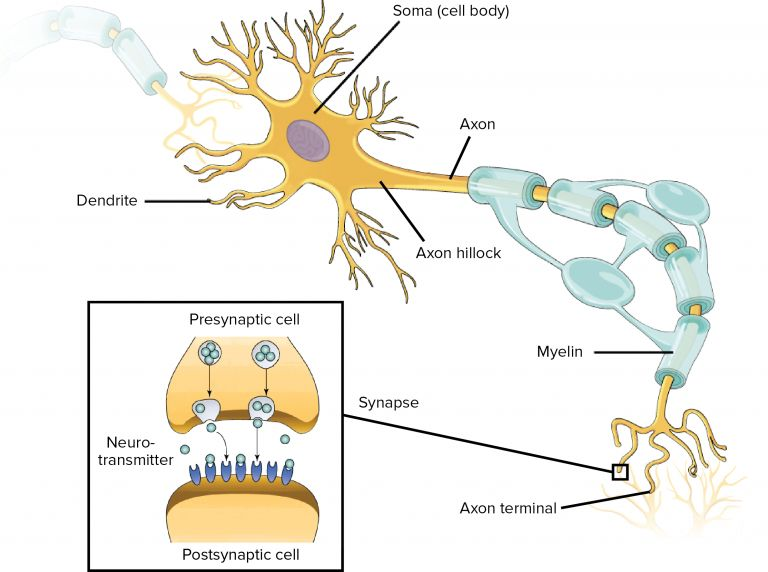
\includegraphics[width=0.7\textwidth]{./data/neural.jpg}
    \caption{Anatomy of the neuron}
    \label{fig:my_picture}
    \vspace{1pt} % Vertical space, optional
    \small{Source: Source:“Neurons and glial cells” by OpenStax College, Biology CC BY-NC-SA 3.0 License.}
\end{figure}


\subsection{Physiology of a Neuron}
\paragraph{The}

 second thing to appreciate about neurons is their specialized physiology — that is the cellular functions of neurons. The most striking feature of neural cellular function is the action potential. This is the mechanism which allows neurons to transmit information reliably over long distances without the transmission attenuating.

\vspace{10pt}
It is important to remember that neurons bathe in an extracellular solution of mostly water, salts and proteins. The forces caused by the movement of salts into and out of the cell and the different concentrations of these salts is the physical basis of the neuron’s remarkable behavior. There are sodium-potassium pumps which move sodium out of the cell and potassium in, so that the concentration of sodium outside the cell is higher than inside and the concentration of potassium outside the cell is lower then inside.

\vspace{10pt}
An action potential is a discrete event in which the membrane potential rapidly rises (depolarizes) and then falls (polarizes). This discrete event is all-or-nothing, meaning that if an action potential occurs at one part of the neurons membrane, it will also occur in the neighboring part, and so on until it reaches the axon terminal. Action potentials do not tend to travel backwards, because, once a section of the membrane has fired an action potential, electrochemical-forces hyper-polarize the region of membrane while the channels which were previously open close and become inactive for some duration of time.

\vspace{10pt}
The action potential is the result of different species of ions traveling across the cell membrane through channels and the activation and inactivation of those channels on different time scales. A stereotypical action potential occurs as follows:

\begin{figure}[H]
    \centering
    \begin{minipage}[b]{0.45\textwidth}
      \centering
      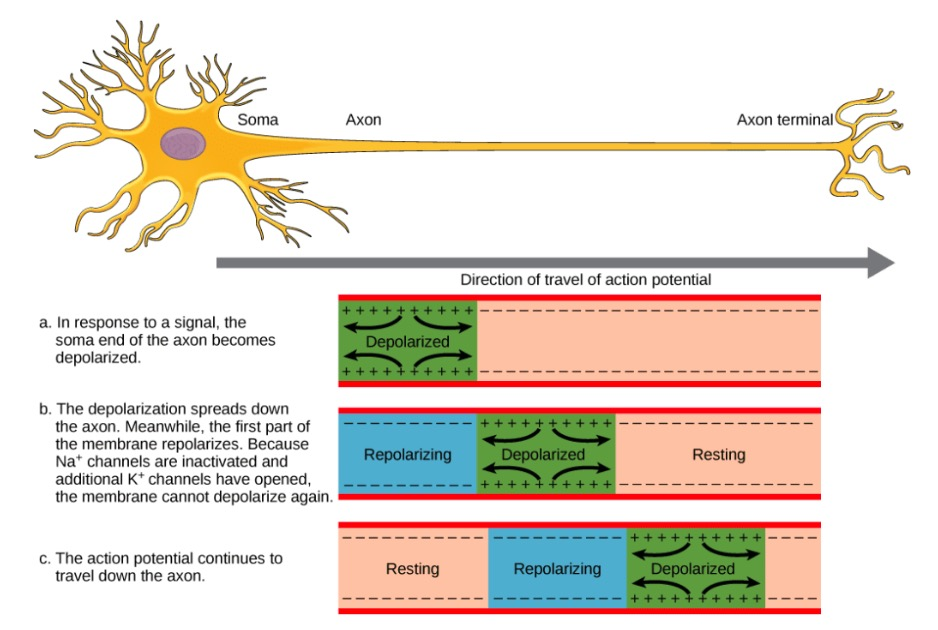
\includegraphics[width=\textwidth]{./data/propagation-of-nerve-impluse.jpg}
      \caption{Propagation of nerve impluse}
      \label{fig:exampleA}
      \vspace{1pt} % Vertical space, optional
      \small{Source: \href{https://opentextbc.ca/biology/chapter/16-2-how-neurons-communicate/}{Opentex}}
    \end{minipage}
    \hfill
    \begin{minipage}[b]{0.45\textwidth}
      \centering
      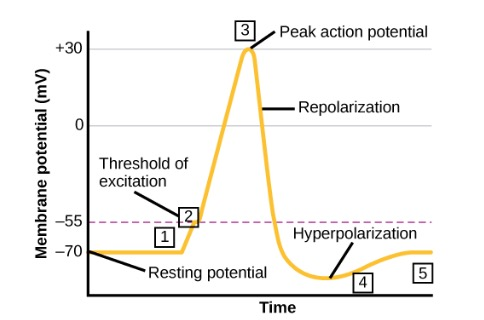
\includegraphics[width=\textwidth]{./data/neuronal-action-potential.jpg}
      \caption{Neuronal action potential}
      \label{fig:exampleB}
      \vspace{1pt} % Vertical space, optional
      \small{Source: \href{https://opentextbc.ca/biology/chapter/16-2-how-neurons-communicate/}{Opentex}}
    \end{minipage}
\end{figure}

\begin{itemize}
    \item \textbf{Equilibrium:} The neuron’s equilibrium membrane potential is near \(-70\) mV — roughly the Nernst Equilibrium of \( E_{K^+} \approx -75 \). At equilibrium, the net current is \(0\) — inward and outward currents are balanced.
    \item \textbf{Depolarization:} Incoming excitatory signals depolarize the membrane. Quick-to-respond voltage gated \( Na^+ \) channels are activated, and \( Na^+ \) rushes in, pushing the membrane potential higher. Slower-to-respond \( K^+ \) channels open, and \( K^+ \) rushes out, pushing the membrane potential lower.
    \item \textbf{Amplification:} If the neuron becomes more stimulated or is stimulated rapidly, many more \( Na^+ \) channels are activated than \( K^+ \) channels. This causes a feedback loop where the influx of \( Na^+ \) causes more \( Na^+ \) channels to activate.
    \item \textbf{Repolarization:} Eventually the membrane potential is near the Nernst Equilibrium of \( Na^+ \) as the sodium channels are maximally open. The slower \( K^+ \) channels catch up to \( Na^+ \), which repolarizes the membrane potential. Meanwhile, the \( Na^+ \) channels become inactive.
    \item \textbf{Hyper-polarization:} \( K^+ \) channels are open while \( Na^+ \) channels are inactive, causing the membrane potential to dip below its typical equilibrium point, near the \( K^+ \) Nernst equilibrium.
    \item \textbf{Refractory Period:} The \( Na^+ \) channels, take a while to become deinactivated, meaning after an action potential, they remain incapable of opening again for a period of time. The period in which most \( Na^+ \) channels are called the absolute refractory period (the neuron cannot spike no matter the strength of the stimulus) while the period in which many \( Na^+ \) channels are inactivated is called the relative refractory period (the neuron can spike given a sufficiently strong stimulus).
\end{itemize}



\subsection{Spike train}

Spike trains are the language of neurons. People tend to think of spikes as point-events and spike trains as point-processe. We describe these with the neural response function:

\begin{equation}
    \rho(t) = \sum_{i=1}^{k} \delta(t-t_i)
\end{equation}

where an impulse is defined as the dirac delta function (which is convenient for counting things):

\begin{equation}
    \delta(t) = \begin{cases} 1 & \text{if } t = 0, \\ 0 & \text{otherwise} \end{cases}
\end{equation}

Often, it is useful for analysis to assume spike trains are generated by random processes. Assuming spikes are independent of each other, we can model this point process is a Poisson process, in which we know the probability n spikes occur in the interval $\Delta T$:

\begin{equation}
    P\{n \text{ spikes occur in } \Delta t\} = \frac{(rt)^n}{n!} \exp(-rt)
\end{equation}

To generate spikes according to a Poisson point process, generate a random number r in a sufficiently small time interval, such that only 1 spike should occur, and check whethe $r < firingRate \Delta T$. However, make sure that $firingRate\Delta T < 1$.






\section{Historical Models}

\subsection{The M-P model}
Since the Spanish anatomist Cajal founded the neuron theory at the end of the 19th century, the biological characteristics and related electrical properties of neurons have been discovered one after another. In 1943, the M-P model of neurons (shown in Figure 1.4) was first proposed in the paper "Logical Activities of Thoughts Contained in Neural Activities" \cite{Mcculloch1854LOGICALCALCULUSIDEAS}. The model was created by psychologists W.S. McCulloch and W.S. McCulloch from the United States. Another mathematician, W.A. Pitts.

\begin{figure}[H]
    \centering
    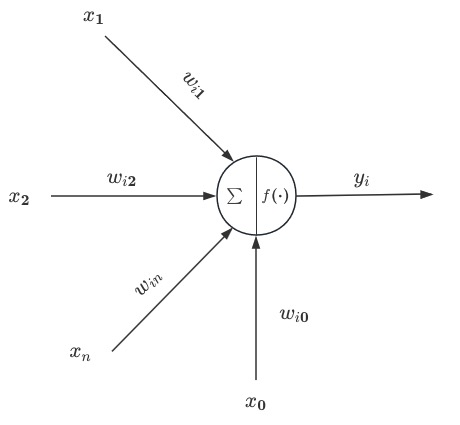
\includegraphics[width=0.9\textwidth]{./data/M-P.jpg}
    \caption{Schematic diagram of the M-P model of neurons}
    \label{fig:my_picture}
    \vspace{1pt} % Vertical space, optional
\end{figure}

In the figure, $x_i$, 1, 2, ..., represents the input signal transmitted from other neurons connected to the current neuron, $w_{ij}$ represents the connection strength or weight from neuron j to neuron i, $\theta_i$ is the neuron The activation threshold or bias of the element, f is called the activation function or transfer function. The output of the neuron $y_i$ can be expressed as follows:

\begin{equation}
    y_i = f(\sum_{j=i}^{n} w_{ij}x_j-\theta_i)
\end{equation}

This model describes neurons from the perspective of logical functional devices, opening up a path for theoretical research on neural networks. The M-P model is a mathematical simplification of the biological neuron information processing model, and subsequent neural network research work is based on it. 



\subsection{Hebb learning rules}
In 1949, in the book "The Organization of Behavior", the psychologist Donald O. Hebb analyzed the change rules of the connection strength between neurons, and based on this, he proposed the famous Hebb learning rule \cite{Hebb2002OrganizationBehaviorNeuropsychological}. Inspired by Pavlov's conditioned reflex experiments, Hebb believed that if two neurons are fired at the same moment, the connection between them should be strengthened. The Hebb learning rule defined based on this is as follows:

\begin{equation}
    w_{ij}(t + 1) = w_{ij}(t) + \alpha y_j(t)y_i
\end{equation}

Among them, $w_{ij}(t+1)$ and $w_{ij}(t)$ represent the connection strength between neuron j and neuron i at time t and t + 1 respectively, while $y_i$ and $y_j$ are the outputs of neurons i and j.


Hebb's rule belongs to the category of unsupervised learning algorithms. Its main idea is to adjust the connection relationship between two neurons according to their excitation state, so as to realize the simulation of simple neural activities. Following the Hebb learning rule, the supervised delta learning rule of neurons was proposed to solve the learning problem of neuron weights when the input and output are known. This algorithm continuously adjusts the connection weights to make the actual output of the neuron consistent with the expected output. Its learning correction formula is as follows


\begin{equation}
    w_{ij}(t + 1) = w_{ij}(t) + \alpha(d_i - y_i)x_j(t)
\end{equation}

Among them, $\alpha$ is the learning rate of the algorithm, $d_i$ and $y_i$ are the expected output and actual output of neuron i, $x_j{t}$represents the state (activation or inhibition) of neuron j at time t.

Intuitively speaking, when the actual output of neuron i is greater than the expected output, the connection weight with the activated neuron is reduced, and the connection weight with the inhibited neuron is increased; when the actual output of neuron i is greater than the expected output If it is small, the connection weight with activated neurons will be increased, while the connection weight with inhibited neurons will be reduced. Through such an adjustment process, neurons will store the correct mapping relationship between input and output in the weight, thus possessing the ability to represent data. The Hebb learning rule and the Delta learning rule are both proposed for a single neuron. The learning rules for parameters in a network composed of neurons will be discussed later. The research work done by the above pioneers paved the way for the emergence of neural computing and inspired many scholars to continue exploring and researching this field.




\subsection{Hodgkin–Huxley model}
The Hodgkin–Huxley model, or conductance-based model, is a mathematical model that describes how action potentials in neurons are initiated and propagated \cite{A.L.Hodgkin1952QuantitativeDescriptionMembrane}. It is a set of nonlinear differential equations that approximates the electrical engineering characteristics of excitable cells such as neurons and muscle cells. It is a continuous-time dynamical system.

\vspace{10pt}
The typical Hodgkin–Huxley model treats each component of an excitable cell as an electrical element (as shown in the figure). The lipid bilayer is represented as a capacitance (\(C_m\)). Voltage-gated ion channels are represented by electrical conductances (\(g_n\), where \(n\) is the specific ion channel) that depend on both voltage and time. Leak channels are represented by linear conductances (\(g_L\)). The electrochemical gradients driving the flow of ions are represented by voltage sources (\(E_n\)) whose voltages are determined by the ratio of the intra- and extracellular concentrations of the ionic species of interest. Finally, ion pumps are represented by current sources (\(I_p\)).

\begin{figure}[h]
    \centering
    
\includegraphics[width=0.9\textwidth]{./data/Hodgkin-Huxley.png}
    \caption{Typical Hodgkin–Huxley model}
    \label{fig:my_picture}
    \vspace{1pt} % Vertical space, optional
    \small{Source: \href{https://en.wikipedia.org/wiki/Hodgkin%E2%80%93Huxley_model}{Wikipedia}}
\end{figure}

\vspace{10pt}
Mathematically, the current flowing through the lipid bilayer is written as:

\begin{equation}
    I_{c} = C_{m} \frac{dV_{m}}{dt} 
\end{equation}

The current through a specific ion channel:
\begin{equation}
    I_{i} = g_{i} (V_{m} - V_{i}) 
\end{equation}


For a cell with sodium and potassium channels, the total membrane current per unit area (I) is given by:

\begin{equation}
    I = C_{m} \frac{dV_{m}}{dt} + g_{K} (V_{m} - V_{K}) + g_{Na} (V_{m} - V_{Na}) + g_{l} (V_{m} - V_{l})
\end{equation}


Where:

\begin{itemize}
    \item \textbf{ I:} is the total membrane current per unit area.
    \item \textbf{$C_{m}$:} is the membrane capacitance per unit area.
    \item \textbf{ $g_{K}$ and $g_{Na}$:} are the potassium and sodium conductances per unit area, respectively.
    \item \textbf{$V_{K}$ and $V_{Na}$:} are the potassium and sodium reversal potentials, respectively.
    \item \textbf{$g_{l}$ and $V_{l}$:} are the potassium and sodium reversal potentials, respectively.
\end{itemize}

The time-dependent elements of this equation are \( V_{m} \), \( g_{Na} \), and \( g_{K} \), where the last two conductances depend explicitly on the membrane voltage (\( V_{m} \)) as well.

\subsection{Mark I perceptron}


In 1958, F. Rosenblatt invented the perceptron model (Perceptron), which was the first model in history to introduce the concept of neural networks into electronic computer processing, marking a new stage in the development of neural networks. The perceptron is a binary linear classification model that determines the output of a two-class model by weighted summation of the input features followed by an activation function. The activation function is a step function, used to determine whether the input value is positive or negative. The mathematical representation of the perceptron model is as follows, where \( x \) represents the input vector, \( w \) represents the weight vector, \( b \) represents the bias term, and \( y \) is the output value, which can be \(+1\) or \(-1\), with the mathematical representation being:


\begin{equation}
    y = f(x) = \text{sign}(w \cdot x + b)
\end{equation}

Here, \( w \cdot x \) represents the dot product of vectors \( w \) and \( x \), and the definition of the \( \text{sign} \) function is as follows:

\begin{equation}
    \text{sign}(x) = 
\begin{cases}
+1, & \text{if } x \geq 0 \\
-1, & \text{if } x < 0
\end{cases}
\end{equation}


The perceptron learning algorithm is based on the principle of reducing the error of classification. When the classification result is incorrect, it adjusts the weights and biases, thus improving the classification ability step by step. The perceptron learning algorithm aims to find the weights and biases that minimize the classification error. Let's define a training set \( T = \{(x_1, y_1), (x_2, y_2), \ldots, (x_n, y_n)\} \), where \( x_i \) is the input vector and \( y_i \) is the corresponding output. The goal of the perceptron learning algorithm is to minimize the loss function \( L(w,b) \):

\begin{equation}
L(w,b) = - \sum_{x_i \in M} y_i (w \cdot x_i + b)
\end{equation}

where \( M \) is the set of misclassified examples. The perceptron updates the weights \( w \) and bias \( b \) to minimize \( L(w,b) \):

\begin{equation}
\min_{w,b} L(w,b) = - \sum_{x_i \in M} y_i (w \cdot x_i + b)
\end{equation}

The gradient descent method is used to update the weights and biases, which aims to adjust the weights and biases in the opposite direction of the gradient of the loss function. The updates for weights \( w \) and bias \( b \) are as follows:

\begin{equation}
\nabla_w L(w,b) = - \sum_{x_i \in M} x_i \cdot y_i
\end{equation}

\begin{equation}
\nabla_b L(w,b) = - \sum_{x_i \in M} y_i
\end{equation}

Therefore, each time an example \( (x_i, y_i) \) is misclassified, the weights \( w \) and bias \( b \) are updated as follows:

\begin{equation}
w_{\text{new}} = w_{\text{old}} + \eta y_i x_i
\end{equation}

\begin{equation}
b_{\text{new}} = b_{\text{old}} + \eta y_i
\end{equation}

where \( \eta \) is the learning rate, a positive constant determining the size of the update step.


In the algorithm, \( 0 < \eta \leq 1 \) is the learning rate. It determines the size of the adjustment to the weights during the learning process. When the perceptron classifies an example correctly, the weights and bias are not adjusted. When it misclassifies an example, it adjusts the weights and bias towards the direction that could possibly correct the error. This process is not changed until all examples are classified correctly, or the process reaches a preset number of iterations. According to the update rules from equations (10) and (11), the weights \( w \) and bias \( b \) are adjusted as follows:

\begin{equation}
w = \sum_{i=1}^{n} a_i y_i x_i
\end{equation}

\begin{equation}
b = \sum_{i=1}^{n} a_i y_i
\end{equation}

where \( a_i = \eta n_i \), and \( n_i \) is the number of times the perceptron misclassified the \( i \)-th example. The perceptron algorithm is named after the psychologist Frank Rosenblatt, who, along with engineers B. Widrow and M. Hoff, adapted the ADALINE (ADAptive LINear Element) from the model of the same name developed by H. Steinbuch.

\subsection{Delta learning rules}

\subsection{Hopfield neural network model}
The next significant advancement in the field of neural networks occurred in 1969 when M. Minsky and S. Papert pointed out the limitations of the perceptron in their book "Perceptrons," demonstrating that it was incapable of processing the XOR problem. However, this criticism also motivated further research into neural networks with additional layers, leading to the development of multilayer networks. The key breakthrough was the introduction of the "backpropagation" algorithm that enabled the training of multilayer networks.

A single-layer perceptron can only solve problems linearly separable because it is essentially a linear classifier. It was realized that to overcome the limitations of the perceptron and solve non-linearly separable problems, one must utilize multilayer networks and non-linear activation functions. The first step in this direction was taken by introducing the concept of a neural network capable of associative memory, which led to the invention of the Hopfield network by J.J. Hopfield in 1982.

The Hopfield network, an energy-based model, is particularly known for solving the Travelling Salesman Problem (TSP). It opened new avenues for using neural networks in optimization problems beyond the domain of traditional computation.

Hopfield's work not only advanced the theoretical foundations of neural networks but also laid the groundwork for the development of modern neural networks, which are capable of learning complex patterns and solving diverse problems. This laid the foundation for significant strides in the field of neural networks, inspiring subsequent developments.

The Hopfield network is characterized by its feedback loops as shown in the figure. In the network, the output of each neuron is fed back into itself and other neurons through a set of resistors. Each neuron has a resistance \( R_i \) and a capacitance \( C_i \), and is connected to other neurons via resistors \( R_{ij} \) (where \( i,j = 1,2,...,n \); \( i \neq j \)). Each neuron's voltage \( U_i \) changes according to the charge \( Q_i \) and its voltage is fed back to itself through a resistor \( R_i \), and to other neurons through resistors \( R_{ij} \), (\( i,j = 1,2,...,n \)) with different resistances. The network follows Kirchhoff's Current Law (KCL), and the voltage change at each neuron is described by the following equation:

\begin{equation}
    \sum_{j=1}^{n} \frac{V_j(t)}{R_j} + I_i = C_i \frac{dU_i(t)}{dt} + \frac{U_i(t)}{R_i}, \quad i = 1, 2, \ldots, n
\end{equation}

However, in a Hopfield network, each neuron's voltage is modified by an activation function \( f \) to produce an output \( V_i \):

\begin{equation}
    V_i(t) = f_i(U_i(t)), \quad i = 1, 2, \ldots
\end{equation}

Then, the state energy of a Hopfield network is defined as:

\begin{equation}
W = R_{i,j}^{-1} (i,j=1,2,...,n)
\end{equation}

where \( R_i' \) are the weights of the network. The energy function of the Hopfield network is given by:

\begin{equation}
    E(t) = -\frac{1}{2} \sum_{i=1}^{n} \sum_{j=1}^{n} \frac{V_i(t)V_j(t)}{R_{ij}} - \sum_{i=1}^{n} V_i(t)I_i + \sum_{i=1}^{n} \frac{1}{R_i} \int_{0}^{V_i(t)} f^{-1}(V) \, dV
\end{equation}

Finally, a Hopfield network adjusts its state iteratively to minimize the energy function \( E(U) \), which leads to stable states—these are the solutions to the problem that the network is trying to solve. The dynamics of a Hopfield network's voltage adjustment towards stable states is analogous to the process of a physical system reaching its lowest energy state.

The Hopfield network is a recurrent neural network, which is to say, it possesses feedback loops. This feature allows it to have dynamic memory. Dynamic memory is different from the static memory seen in the perceptron, which only allows for the storage of a fixed set of patterns. The Hopfield network can store a variety of patterns and retrieve them based on the input, making it a form of associative memory.

Hopfield's paper not only triggered the renaissance of interest in neural networks but also led to the exploration of new types of neural networks. One significant development in this area was the Boltzmann machine, introduced by G.E. Hinton, T.J. Sejnowski, and D.H. Ackley in 1983. This machine was an extension of the Hopfield network and could solve problems that Hopfield networks could not.

\subsection{Boltzmann machine}

A Boltzmann machine is similar to a Hopfield network in that it is a network of units with a global energy function. However, unlike the Hopfield network, a Boltzmann machine has stochastic units and operates based on probabilistic rather than deterministic rules. This means that a Boltzmann machine can escape from local minima, a feature that is particularly beneficial when dealing with optimization problems.

A special case of the Boltzmann machine is the Restricted Boltzmann Machine (RBM), which constrains the connections between units to form a bipartite graph. This constraint simplifies the learning algorithm and makes it more efficient. RBMs have found a wide range of applications, particularly in the development of deep learning algorithms. For instance, they can be used to pre-train the layers of a deep neural network, improving the efficiency and effectiveness of the training process.

The collaborative work of Hinton and his colleagues on Boltzmann machines and the development of efficient training algorithms have played a vital role in the evolution of neural networks. Their work has paved the way for the deep learning revolution, which is now at the forefront of artificial intelligence research and applications.





\section{Applications}
Biological neural network modeling is pushing the technological frontier in every field by simulating biological neural networks, solving real-world challenges, and improving the quality of human life. These applications demonstrate the power of interdisciplinary collaboration, bringing together biology, computer science, engineering and medicine to advance the future of medical technology and technology.

\begin{itemize}
    \item \textbf{ Brain-Computer Interface (BMI):} Brain-computer interface technology allows the human brain to interact directly with external devices, which has significant potential in providing assistive tools and restoring limb movement to paraplegic patients. Through the application of biological neural network models, researchers can better understand how brain signals map to body movements and how these signals can be interpreted to control external devices. These models also help improve algorithms to decode and translate brain activity into mechanical movements or electrical signals, enhancing the accuracy and responsiveness of brain-computer interfaces.
    \item \textbf{AI:} Biological neural networks provide artificial intelligence with a framework that mimics complex brain processing functions, particularly in the areas of vision and language processing. Deep learning, a biologically inspired algorithm, has led to breakthroughs in image recognition, speech-to-text conversion, and machine translation. Advances in these technologies, due in part to the understanding and simulation of how biological neural networks work, are changing the way we interact with technology and are finding applications in areas such as medicine, self-driving vehicles and smart homes.
    \item \textbf{Cognitive and Behavioral Research:} Biological neural network modeling helps scientists understand how cognitive processes are encoded in the brain. Such models can simulate memory formation, attention control, and decision-making processes, providing insights into studying behavior in humans and other animals. Additionally, they play an important role in explaining cognitive patterns in mental health conditions such as anxiety, depression, and other psychological disorders.
    \item \textbf{Precision medicine and disease diagnosis:} In the field of precision medicine, modeling of biological neural networks can predict how individuals will respond to specific treatments, thereby enabling personalized medicine. By analyzing a patient's gene expression data, protein levels and other biomarkers, the model is able to predict the course of the disease and the patient's response to drug treatment. Such models can also reveal new disease mechanisms, guide the development of future treatment strategies, and help physicians design customized treatment regimens to maximize efficacy and reduce side effects.
\end{itemize}



% 人类通过研究碳基生物制造硅基生物

%----------------------------------------------------------------------------------------
\clearpage
\bibliographystyle{unsrt} % This specifies the style of the bibliography
\bibliography{/Users/dengkai/workspace/papers/latex/config/ref} % This should match the name of your .bib file without the extension
\end{document}

